% \section{Wettbewerbsanalyse}

Das Ermitteln und Priorisieren aller relevanten Kundenanforderungen ist ein kontinuierlicher und unerlässlicher Vorgang, um zum einen die Bedürfnisse der zukünftigen Nutzer erfüllen zu können und zum anderen, um das Produkt langfristig wettbewerbsfähig zu gestalten. Hierfür ist es essenziell, sich mit Wettbewerbern, ihren Produkten und vermeintlichen Strategien auseinandersetzten. Erst dies bildet die Grundlage die eigenen Chancen auf dem Markt zu bewerten und mögliche Alleinstellungsmerkmale (\engl unique selling point, USP) zu ermitteln, um sich von Wettbewerbern frühzeitig abzusetzen. Zusätzlich zeigt die Analyse, welche Features bereits auf dem Markt im Einsatz sind und vom User \ggf schon als grundlegende Features erwartet werden.

Die Durchführung der Wettbewerbsanalyse erfolgte in den folgenden Einzelschritten:

\begin{itemize}
    \item Ermittlung der Hauptwettbewerber
    \item Erstellung eines Konkurrenzprofils
    \item Darstellung der einzelnen Wettbewerber
    \item Bewertung der strategischen Ausrichtung
    \item Zusammenfassung
\end{itemize}

\subsection{Ermittlung der Hauptwettbewerber}

Für die Ermittlung der bedeutendsten Mitbewerber ist es erforderlich die Hauptmerkmale und Ziele des eigenen Dienstes, für einen Abgleich mit den potenziellen Wettbewerbern, gut zu kennen. Hierbei ist zu berücksichtigen, dass es in der digitalen Welt selten Wettbewerber gibt, die 1:1 den gleichen Dienst anbieten \bzw die gleiche Strategie verfolgen. Jedoch können hierbei mittelfristig vollwertige Konkurrenzprodukte entstehen, die zum Zeitpunkt der Analyse nur wenige gemeinsame Parallelen oder Features aufgewiesen haben.

Digital Home Town (DHT) setzt in seiner langfristigen Ausrichtung auf die Stärkung des lokalen/ regionalen Raums mit seinen sozialen Verflechtungen. Dies soll geschehen durch die Förderung des digitalen Austauschs zwischen allen Menschen und Institutionen, die das örtliche Dasein widerspiegeln. Die Schwerpunkte von DHT sind wie folgt:

\begin{enumerate}
    \item Das Vernetzen von Personen, die das gleiche Interesse oder ähnliche Bedürfnisse teilen, einen Austausch von \bspw Informationen, Waren \usw anstreben oder Unterstützung/ Hilfestellung suchen.
    \item Die Stärkung lokaler Vereine und/ oder Dienstleistungen, damit diese ihre Angebote gezielter darstellen und leichter mit Interessierten in Kontakt treten können.
    \item Die Unterstützung öffentlicher Einrichtungen, um einen leichteren Zugang \ua zu amtlichen Informationen, Terminen \usw zu ermöglichen.
\end{enumerate}

Zugleich sieht sich DHT allen Personen verpflichtet und strebt einen barrierefreien Zugang an.

Abgeleitet aus der Zielsetzung von DHT konnten eine Reihe von Web-Diensten ermittelt werden, die sich \ua auf den lokalen Raum in Bezug auf Austausch, Vernetzung oder Zusammenführung privater Parteien konzentrieren. Als besonders etablierte und aktive Vertreter in mindestens einem der genannten Bereiche konnten zunächst

\begin{itemize}
    \item Facebook,
    \item Nebenan.de,
    \item Spontacts,
    \item eBay Kleinanzeigen und
    \item Doctolib
\end{itemize}

ausfindig gemacht werden. Im weiteren Verlauf werden exemplarisch nur die Social-Networking-Vertreter weiter ausgeführt. Dies betrifft demnach nicht Doctolib, da es sich eher um eine spezialisierte Software für E-Health-Angebote handelt.

\subsection{Konkurrenzprofil}

Zur detaillierten Auseinandersetzung mit den ermittelten Wettbewerbern ist es erforderlich ein Profil jedes einzelnen zu erstellen. Dieses sogenannte Konkurrenzprofil gibt in der Gegenüberstellung mit dem eigenen Selbstprofil eine transparente Bewertungsbasis, mit dessen Hilfe wertvolle Erkenntnisse über die Stärken, Potenziale und strategischen Ziele abgeleitet werden können.

Für den Vergleich werden die folgenden Punkte gesondert betrachtet:

\begin{itemize}
    \item Fokus des Dienstes und dessen Zielgruppe,
    \item Möglichkeiten der Selbstdarstellung und des Austausches,
    \item Benachrichtigungen über Änderungen und Neuigkeiten und
    \item Entdecken von Inhalten.
\end{itemize}

\subsection{Kurzdarstellung}

\subsubsection{Facebook}

Facebook ist ein etablierter und weltweit verbreiteter Dienst, der es ermöglicht sich mit Menschen aus der ganzen Welt zu vernetzen, miteinander in Kontakt zu bleiben und Inhalte aus dem eigenen Leben mit anderen zu teilen.
In den frühen Jahren von Facebook waren insbesondere Studenten die anvisierte Zielgruppe, welche über die Jahre jedoch breiter geworden und mittlerweile sehr heterogen ist.

\begin{figure}
    \centering
    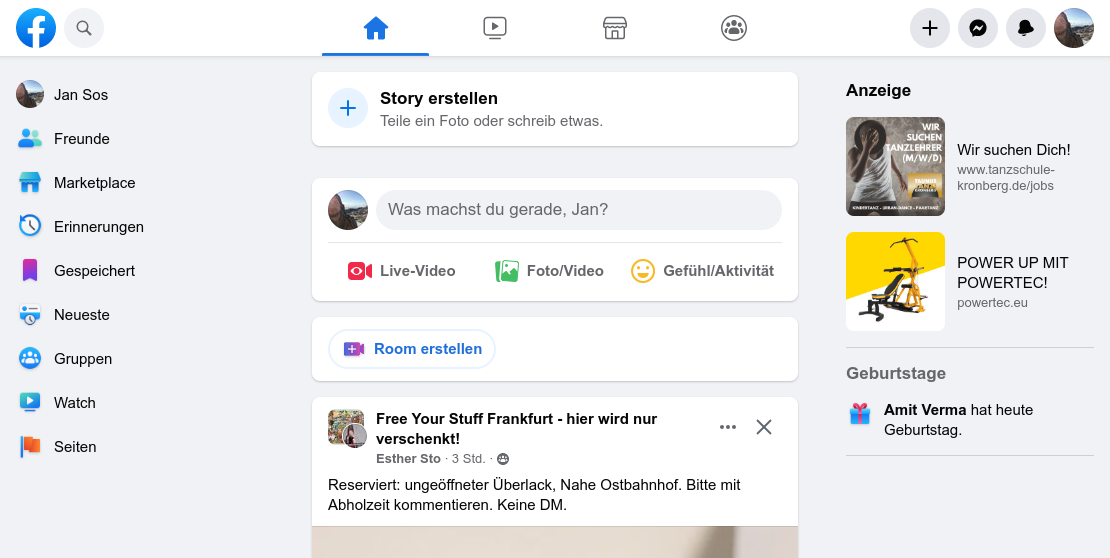
\includegraphics[width=\textwidth]{figures/jan/pic_facebook.png}
    \caption[Startseite von Facebook]{Startseite von Facebook}
    \label{fig:facebook}
\end{figure}

Die Nutzung von Facebook kann je nach Bedürfnissen des Einzelnen sehr verschieden sein. Hier bietet Facebook neben reinen Darstellungs- und Austauschmöglichkeiten eine Bandbreite an Anwendungen an, wie \ua integrierte Video-, Games- und Dating-Portale und ein eigenes Bezahlsystem, auf welche hier im weiteren Verlauf nicht weiter eingegangen wird.

\paragraph{Selbstdarstellung}

Zur Darstellung einer Organisation, einer öffentlichen oder privaten Person, bietet Facebook je nach Typ ein eigenes Profil an, auf welchem \ua Bilder, persönliche Informationen und Vorlieben, wie \zB Musik öffentlich dargestellt werden können. Inwieweit diese Inhalte einsehbar sind, ist individuell einstellbar. Zusätzlich zu den statischen Informationen beinhaltet das Profil noch eine Pinnwand, auf welcher ältere und aktuelle Beiträge listenmäßig aufgeführt sind.

\paragraph{Formen des Austausches}

Für den interaktiven Austausch und das Teilen von Momenten dienen Beiträge (Posts) . Diese können von jedem verfasst und auf der eigenen sowie fremden Pinnwand angebracht werden. Diverse Ereignisse, wie \bspw das Hochladen von neuen Bildern, generieren systematisch einen eigenen Beitrag, um Bekannte, Follower \etc über eine Neuigkeit auf dem Profil zu informieren. Die Beiträge können wiederum von Anderen kommentiert oder mittels eines Icons bewertet werden. Zudem können sie neben einfachem Text auch Bilder oder Videos enthalten und lassen sich mittels Tags (Orte, GPS, Veranstaltungen, Personen, \ldots) genauer spezifizieren.

Für den Austausch mit mehreren Personen bietet Facebook Gruppen an. Dort können sich Anwender über gemeinsame Themen austauschen. Gruppen haben wie Profile einen statischen Teil, in dem die Admins im Freitext eine Kurzbeschreibung der Gruppe verfassen und veröffentlichen können. Darüber hinaus verfügen Gruppen auch über eine Pinnwand, über die die Mitglieder miteinander im Austausch stehen. Gruppenmitglieder können darüber hinaus auch Events erstellen, an welchen die Mitglieder teilnehmen können.
Gruppen werden sehr häufig und für verschiedene Themen verwendet. Sie dienen besonders im städtischen Raum \bspw zum Verschenken von ungenutzten Dingen (Free your Stuff), zum Finden von neuen Kontakten in einer neuen Stadt (New in Munich) oder das Finden von Menschen in der Nähe mit ähnlichen Hobbies (\zB Wandern). Auch der überregionale/ internationale Austausch über diverse Themen in unterschiedlichen Bereichen ist weit verbreitet.

Der Austausch materieller Gegenstände findet neben den einzelnen Gruppen hauptsächlich auf einem digitalen Marktplatz statt. Die geschalteten Anzeigen enthalten eine Überschrift, freie Beschreibungen, Bilder, Angaben über den Zustand, Preisvorstellung, Ort und den Herausgeber der Anzeige. Bei der Erstellung dieser muss der Verfasser die Anzeige einer vordefinierten Kategorie zuweisen, um die Auffindbarkeit zu erleichtern. Für den Interessenten besteht neben der direkten Kontaktaufnahme die Möglichkeit sich die Anzeige zu merken, sie mit einem Kontakt zu teilen oder einen Alarm zu erstellen, sobald ähnliche Produkte angeboten werden.

Zur Pflege von Kontakten ist es in Facebook möglich, Personen bei gegenseitigem Einverständnis in eine Kontaktliste aufzunehmen. Mithilfe dieser sogenannten Freundesliste können Inhalte selektiv verteilt werden. Für Personen, die nicht in der Kontaktliste enthalten sind, sind diese Inhalte nicht sichtbar. Darüber hinaus werden befreundete Personen über das Dashboard gezielter informiert, sobald ein Kontakt aus der Liste eine Aktivität durchgeführt hat.

Für den direkten und nicht öffentlichen Austausch wird dem Anwender ein Chat angeboten, in welchem 1:1- und Gruppenchats stattfinden können. Der Nachrichtenaustausch findet hierbei in Echtzeit statt. Die Nachrichten können analog, wie Beiträge, die gleichen Inhalte aufweisen (Bilder, Links \etc). In 1:1-Gesprächen ist es darüber hinaus auch möglich, Sprach- und Videoanrufe zu tätigen.

\paragraph{Neuigkeiten}

Um bei der Vielzahl der Beiträge und Reaktionen von Freunden oder in Gruppen den Überblick zu behalten, werden auf einem Dashboard Neuigkeiten in Form einer endlosen und unsortierten Liste angezeigt. Darüber hinaus beinhaltet das Dashboard kommerzielle Werbung und Beiträge von noch nicht abonnierten Gruppen, die für den Nutzer von Interesse sein könnten.

Neben dem Dashboard gibt es zusätzlich noch eine Notifications-Seite, welche einen gezielteren Fokus aufs Wesentliche ermöglicht. Notifications sind kurze Benachrichtigungen, die gesammelt in einer Liste abgelegt werden. Sie beinhalten \ua Geburtstage der Kontakte, bevorstehende angemeldete Events, neue Beiträge aus abonnierten Gruppen sowie Reaktionen auf eigene oder kommentierte Beiträge.

\paragraph{Recherche}

Zur Findung von Personen, Gruppen \usw existiert eine Suchfunktion, mit deren Hilfe alle FB-Inhalte durchsucht werden können. Mit dem Suchfilter können auch die Art der Inhalte, Verfasser, Gruppen, Zeitraum \uvm genauer spezifiziert werden.

Das Sichern von Beiträgen und öffentlichen Profilen kann ebenso vorgenommen werden. Das Speichern erfolt direkt am Objekt.
Gespeicherte Beiträge und öffentliche Profile können im Anschluss auf einer separaten Seite je nach Typ aufgelistet und dort auch verwaltet werden.

\subsubsection{Nebenan.de}

Nebenan.de ist ein im Jahr 2015 in Betrieb genommenes Portal, welches wie Facebook seinen Mehrwert im Vernetzen von Menschen sieht. Anders als Facebook fokussiert es sich dabei ausschließlich auf die unmittelbare Nachbarschaft des Anwenders.

\begin{figure}
    \centering
    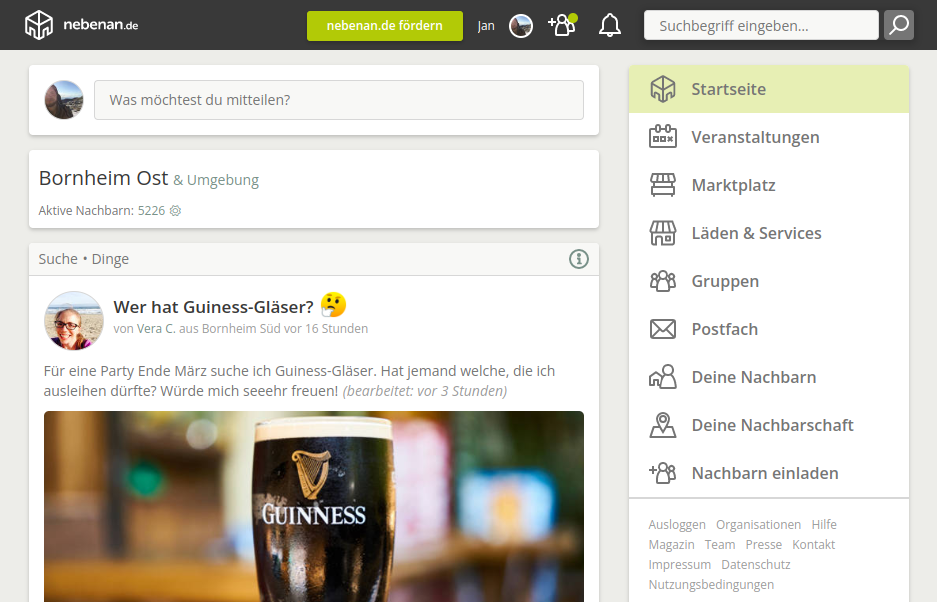
\includegraphics[width=\textwidth]{figures/jan/pic_nebenan.png}
    \caption[Startseite von nebenan.de]{Startseite von nebenan.de}
    \label{fig:nebenan}
\end{figure}

Die Zielgruppe besteht daher aus allen in der Nachbarschaft vorkommenden Interessengruppen, wie \zB Bewohner, Vereine, Firmen und Organisationen. Die Nachbarschaftsgrenze wird durch die eigene Adresse vom System definiert und kann nicht individuell angepasst werden. Ein Austausch über die Nachbarschaftsgrenze hinaus ist nicht möglich, was den Fokus auf die Stärkung und Belebung der Nachbarschaft deutlich hervorhebt.

\paragraph{Selbstdarstellung}

Für die Darstellung existieren in Nebenan.de zwei Arten von Profilen. Die erste Profilart gilt Einzelnutzern. Hierbei können sich Anwohner über ein Kurzprofil mit Foto, einem Freitext sowie ihren Interessen und Angeboten vorstellen. Zur Auswahl der Interessen und Angebote stehen fest definierte Vorschläge zur Verfügung. Angebote beschreiben neben den Interessen, was der Anwohner bereit ist, in seine Nachbarschaft einzubringen. Dies könnte \bspw Pakete annehmen, Blumen gießen, Fahrrad reparieren oder Gesellschaft leisten sein.
Neben der eigenen Darstellung zeigt das Profil die Aktivität des Anwohners an. Dies beinhaltet \bspw die Auflistung von beigetretenen nebenan-Gruppen und die Anzahl der erhaltenen virtuellen Dankeschöns.
Die zweite Profilart wird von Organisationen und Läden/ Services genutzt, die vor Ort angesiedelt sind und zum alltäglichen Leben in der Nachbarschaft beitragen. Diese Profile sind im Vergleich zu den Anwohnerprofilen mit deutlich mehr Informationen ausgestattet. Jedes dieser Profile muss beim Anlegen mit einer Kategorie versehen werden. Dies kann im Beispiel eines Geschäftes \zB Restaurant, Reisen oder Sport und im Fall einer Organisation Non-Profit, Political Party, Nachbarschafts-Initiative \usw sein. Neben Name, Adresse, Kontaktdaten und Öffnungszeiten können auch zukünftige Ereignisse/ Events, Gesuche, Bekanntmachungen, das Verkaufsangebot und weitere Informationen hinterlegt werden. Die Anwohner können darüber hinaus ihre eigenen Erfahrungen mit der Organisation oder dem Laden sowie Empfehlungen auf deren öffentlichen Profilen kundtun.

\paragraph{Formen des Austausches}

Als zentrales Mittel für den Austausch wird bei nebenan.de der Beitrag genutzt. Dieser kann nach dem Veröffentlichen von allen Anwohnern kommentiert und positiv bewertet werden. Ein Beitrag wird bei der Erstellung mit einer Kategorie versehen. Anhand dieser wird festgelegt, ob es sich bei dem Beitrag um etwas Allgemeines, ein Gesuch, ein Angebot, eine Empfehlung oder ein Event handelt. Jede Kategorie wird des Weiteren zur besseren Einordnung noch in eine oder mehrere aufeinander aufbauende Unterkategorien unterteilt. Je nach Art werden die Beiträge neben der öffentlichen Wand zusätzlich an diverse Seiten wie \zB den Event-Feed im Marktplatz der Nachbarschaft angeheftet.
Die Beiträge bestehen wie bei Facebook klassisch aus einem Titel und einem Freitext und können optional mit Bildern versehen werden. Zusätzlich können je nach Art noch weitere Felder wie \zB Datum und Ort bei Veranstaltungen vorhanden sein.

Die Beiträge des Marktplatzes werden neben der Kategorie Angebot noch in die Unterkategorien Help, Give, Rent, Trade \usw unterteilt. Der Inhalt eines Verkaufsangebots kann des Weiteren noch mit einer Angebotskategorie, wie Food, Baby \& Children, Pets \usw, versehen werden. Alle Angebote werden gesammelt in einer Liste dargestellt und können nach ihrer Angebotskategorie gefiltert oder mit der globalen nebenan.de-Suchfunktion nach Wörtern durchsucht werden.

Für den Austausch von Personen mit gleichen Interessen können in nebenan.de Gruppen erstellt werden, deren Zweck durch einen Gruppennamen und einen Freitext genauer ausgeführt werden kann. In den Gruppen können verschiedene Arten von Beiträgen (Mitteilung, Suche, Angebot, Veranstaltung, \ldots) abgesetzt werden. Diese werden an der Gruppenpinnwand angezeigt und können von allen Gruppenmitglieder kommentiert werden. Die Gruppenfunktion findet jedoch auf nebenan.de nur eine geringe Beachtung.

Eine Chatfunktion für den direkten Austausch mit einzelnen Nutzern ist ebenso integriert. Neben dem reinen Text und Emoticons können mit ihr zusätzlich noch Fotos und Empfehlungen versandt werden.

\paragraph{Neuigkeiten}

Zur Benachrichtigung von neuen Beiträgen gibt es das Dashboard. Hier werden alle Arten von Beiträgen mit Ausnahme der Angebotsbeiträge (Give) nach der letzten Änderung sortiert angezeigt. Der Austausch mit der Nachbarschaft passiert maßgeblich über das Dashboard, wo reinkommende Beiträge entdeckt und beantwortet werden können.
Für den besseren Überblick werden durch Benachrichtungs alle Beiträge, bei denen man selbst aktiv teilgenommen hat und sich neue Ereignisse ergeben haben, nochmal separat aufgelistet.. Darüber hinaus werden auf dem Benachrichtungs-Feed alle Events angezeigt, die zukünftig in der Nachbarschaft stattfinden.

\paragraph{Recherche}

Für die Suche von Beiträgen jeglicher Art steht die nebenan-Suche zur Verfügung. Über diese können anhand eines Freitextes die Beiträge der Nachbarschaft durchforscht werden.
Beiträge, die dem User besonders zusagen oder für ihn wichtige Informationen enthalten, können als Bookmark gespeichert werden und auf der Bookmark-Seite unter Feed oder Marktplatz eingruppiert eingesehen und wieder gelöscht werden.

\subsubsection{Spontacts}

Gegenüber Facebook und Nebenan.de legt Spontacts sein Augenmerk ausschließlich auf das Verabreden/ Treffen für Freizeitaktivitäten von Menschen, die in der gleichen Region wohnen. Spontacts richtet sich an Menschen, die Interesse an bestimmten Aktivitäten haben und dazu neue Kontakte suchen.

\begin{figure}
    \centering
    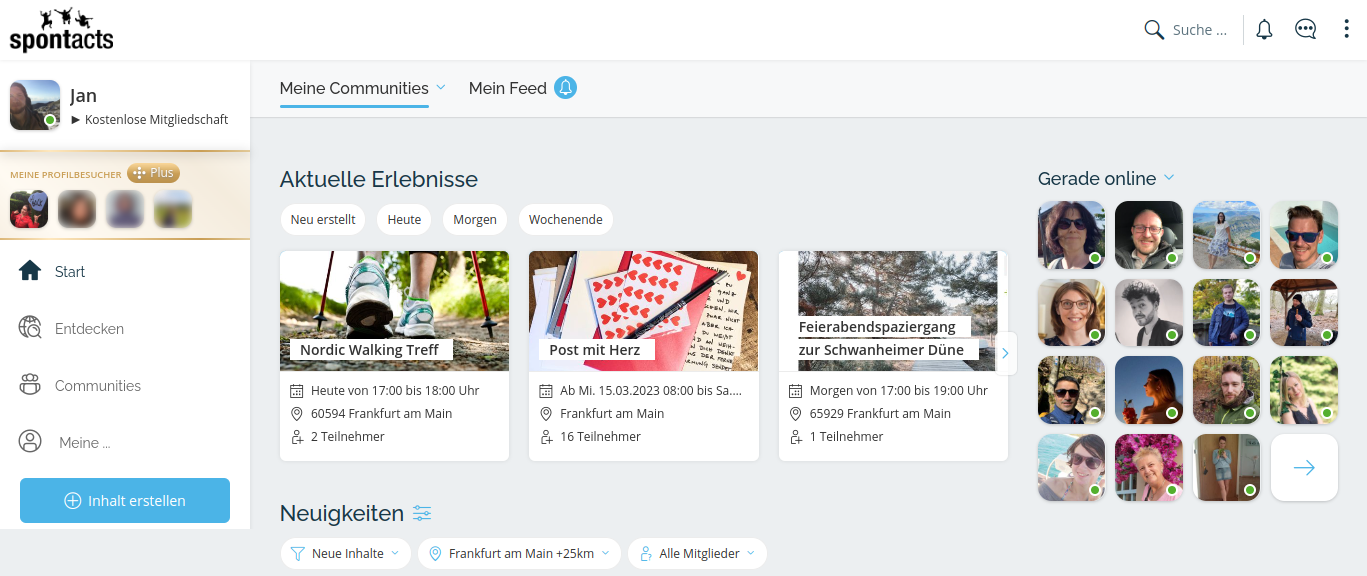
\includegraphics[width=\textwidth]{figures/jan/pic_spontacts.png}
    \caption[Startseite von Spontacts]{Startseite von Spontacts}
    \label{fig:spontacts}
\end{figure}

Der Anwender kann hierfür an erstellten Veranstaltungen teilnehmen oder selbst welche erstellen. Im Gegensatz zu den bereits vorgestellten Diensten besitzt Spontacts einen kostenlosen sowie kostenpflichtigen Account. Ein weiterer Unterschied liegt darin, dass regelmäßig Angebote für die Nutzer von bei Spontacts Angestellten bereitgestellt werden und es sich dadurch nicht um reinen User-Content handelt.

\paragraph{Selbstdarstellung}

Die Benutzer von Spontacts können, wie auch in vergleichbaren Anwendungen, zur Präsentation ihrer Person ein Profil erstellen. Das Grundprofil setzt sich aus Name, Profilbild, Alter und Wohnort zusammen und kann mit weiteren Informationen wie \bspw präferierte Kontakte - für Freizeit, Sport, Reisen, Tanzen und Dating - oder mit zusätzlichen Profilabschnitten (Hobbies, Interessen/ Vorlieben \usw) angereichert werden. In einem weiteren Abschnitt können vergangene und zukünftige Aktivitäten des Users sowie seine Gruppenmitgliedschaften eingesehen werden.

\paragraph{Formen des Austausches}

Zur Interaktion mit anderen Benutzern dienen Beiträge. Diese Beiträge werden je nach Art als einfacher Beitrag, als Aktivität oder als Frage/ Diskussion abgesetzt und anschließend in Communities, Gruppen oder \ggf in Foren angezeigt und können wie gewohnt kommentiert, gelikt und geteilt werden.

Die Communities beschreiben als eine Obergruppe einen Themenbereich (Ausgehen \& Party, Essen \& Trinken, Natur \& Umwelt \usw), zu welchem der Beitrag zugeordnet wird. Beim Erstellen einer Gruppe muss hierfür immer eine passende Community ausgewählt werden.
Anders als bei den anderen vorgestellten Diensten, stellen die Gruppen auf Spontacts das zentrale Feature der Anwendung dar. Diese ähneln vom Funktionsumfang den FB-Gruppen und sind lediglich in ihrem Aufbau anders strukturiert. In ihnen kann sich der Anwender über das Gruppenprofil mit Kurzbeschreibung, Mitgliederanzahl \usw informieren, über eine Pinnwand alle Beiträge der Mitglieder durchstöbern sowie die geplanten Veranstaltungen der Gruppe einsehen.

Für Auseinandersetzungen über die Beiträge hinaus kann mit jedem Anwender eine private Unterhaltung über den Chat geführt werden. Mit dem Chat können Textnachrichten ohne Emoticons, Bilder \etc versendet werden.

\paragraph{Recherche}

Zum Entdecken von Beiträgen, Veranstaltungen, Gruppen, Mitgliedern \uvm bietet eine Suchfunktion je nach zu suchendem Typ weitere Filterfunktionen. Der Anwender kann neben den allgemeinen Einstellungen wie Suchbegriff, Umkreis, Erstelldatum und Community die Anfrage noch mit objektspezifischen Kriterien wie Datum, Alter und ähnliches verfeinern.

Die während der Nutzung des Portals oder während eines Treffens entdeckten Mitglieder können in die Kontaktliste oder Merkliste aufgenommen werden. Die Merkliste ist eine private Liste von Personen, die der Anwender als merkenswert empfand. Die Kontaktliste ist hingegen öffentlich und zur Aufnahme muss eine Anfrage an die Person versendet und bestätigt werden.
Darüber hinaus kann man Mitgliedern folgen, um ihre Aktivitäten besser verfolgen zu können. Wer wem folgt kann jeder Benutzer im jeweiligen Profil einsehen.

\paragraph{Neuigkeiten}

Um innerhalb der Plattform auf dem Laufenden zu bleiben, gibt es wie bei den anderen Portalen ein Dashboard und einen Benachrichtigungs-Feed.
Im Dashboard werden in der Rubrik „Neuigkeiten“ alle anstehenden Veranstaltungen und aktuellen Inhalte aus den gewählten Communities dargestellt. Unter der Rubrik \glqq Mein Feed\grqq\ im Dashboard können
hingegen alle Veränderungen in beigetretenen Gruppen eingesehen werden. Hierzu zählen insbesondere neue Mitglieder und neue Veranstaltungen.
Der Benachrichtungs-Feed enthält neue Kontaktanfragen, Beiträge aus den Gruppen und Plattform News.

\subsection{Strategische Ausrichtung}

Die drei untersuchten Hauptwettbewerber weisen als soziale Netzwerke insbesondere in ihren Features, wie das Vorhandensein von Profil, Chat, Gruppen \usw, viele Gemeinsamkeiten auf. In ihrer strategischen Ausrichtung unterscheiden sie sich jedoch teils stark voneinander.
Facebook ist eine sehr aktive Plattform. Sie unterstützt ganz allgemein das Vernetzen von Menschen mit beliebigen Interessen, Themen und Bedürfnissen. Es fokussiert sich dabei nicht auf einen geografischen Raum oder schränkt die Anwender in irgendeiner Form ein, die einen Austausch verhindern würde. Ein Ausbau oder eine intensive Weiterentwicklung an der Plattform konnte in der vergangenen Zeit nicht wahrgenommen werden \bzw dieser fand nur im Hintergrund statt. Lang- und mittelfristig ist hierbei keine Veränderung zu erwarten, da sich der Konzern hinter Facebook maßgeblich der Entwicklung von zukünftigen Produkten im 3D-Umfeld gewidmet hat.

Nebenan.de ist in seiner bisherigen Ausrichtung der größte Konkurrent für DHT. Die Plattform bietet die Möglichkeit sich innerhalb der eigenen Nachbarschaft zu verschiedenen Themen auszutauschen und zu vernetzen. Der Fokus liegt hierbei auf der Stärkung des Miteinanders in einem lokalen Raum. Die große Herausforderung, die vor Nebenan.de liegt, ist maßgeblich der Aufbau von lokalen Communities, in welchen sich alle gesellschaftlichen Schichten und Altersklassen angesprochen fühlen. Ein weiteres Vorhaben könnte zugleich auch der Ausbau der Plattform sein, um zum einen diese intuitiver zu gestalten sowie zum anderen einen zielgerichteteren Austausch zu ermöglichen.

Spontacts fokussiert sich hingegen sehr stark auf das Vernetzen von Menschen zur Durchführung gemeinsamer Aktivitäten im privaten Bereich. Die Plattform hat eine rege Community. Die Anwender sind in der Lage beliebige Inhalte zu erstellen und an allen Veranstaltungen innerhalb Spontacts teilzunehmen. Harte lokale Einschränkungen \bzgl der Sichtbarkeit von Inhalten existieren wie auch bei nebenan.de nicht.
Die Inhalte der Seite werden darüber hinaus noch durch lokal ansässige Moderatoren betreut. Die Moderatoren erstellen ergänzend weitere Veranstaltungsangebote und führen diese zugleich auch durch. Strategisch versucht Spontacts zunehmend kostenpflichtige Accounts einzuführen, über welche zusätzliche Funktionen, wie \bspw bessere Filterfunktionen, den Anwendern zur Verfügung stehen. Ein weiterer Schritt, um sich weiter auf dem Markt zu etablieren, wäre es die bisherige Zielgruppe - alleinstehend und \ca 30-50 Jahre - zunehmend weiter anzusprechen.

\subsection{Zusammenfassung}

Mithilfe der durchgeführten Analyse der Wettbewerber konnte verdeutlicht werden, dass die untersuchten Dienste alle verschiedene Motivationen sowie Zielgruppen verfolgen. Zugleich verfolgt keiner den Ansatz sich, wie DHT, gezielt auf die Region/ Gemeinde zu konzentrieren, um dort die Vernetzung und den Austausch zu fördern. DHT schließt hierbei die Lücke, die sich zwischen FB als weltweiter Akteur und nebenan.de mit reinem Nachbarschaftsfokus auftut. Absetzen tut sich DHT neben dem örtlichen Bezug auch durch die Einbindung von Vereinen und öffentlichen Organen, die die Plattform zur Kommunikation mit den Anwohnern nutzen können.

Ein weiterer Aspekt, der im direkten Vergleich deutlich wird, ist, dass die Bedienung und das Zurechtfinden auf den Plattformen sehr unterschiedlich ausfallen. Teils sind die Inhalte sehr versteckt, teils sind die zugrunde liegenden Konzepte nicht selbsterklärend gestaltet. Durch den Anspruch von DHT für alle von jung bis alt (generationsübergreifend) verständlich zu sein, ist es essenziell für den Erfolg von DHT, eine Plattform zu entwerfen, die in der Handhabung einfach und intuitiv ist.

Die Analyse zeigt am Beispiel von nebenan.de und Spontacts auch, dass der Aufbau und das Etablieren eines sozialen Netzwerkes viele Herausforderungen mit sich bringen. Als Vorreiter ist Facebook sehr weit in der Gesellschaft verbreitet und ermöglicht durch sein breites Angebot an Features diese für verschiedene Bedürfnisse zu nutzen.
Dies stellt insbesondere neuere Plattformen - wie Nebenan.de und Spontacts - im Aufbau einer Community vor große Herausforderungen, da sie als Newcomer ohne Community und Content mit meist den gleichen FB-Features den Anwender überzeugen müssen, sodass ihre Plattform einen spürbaren Mehrwert gegenüber FB liefert. Dies ist besonders bei Plattformen schwierig, bei denen die Inhalte ausschließlich von den Nutzern erstellt werden. Der Aufbau einer solchen Community ist als besonders zäh anzusehen, da neue Nutzer sich aus Mangel an aktuellen Inhalten schnell wieder von der Plattform abwenden.
Das kontinuierliche Vorhandensein von neuen Inhalten ist ein essenzieller Bestandteil, um ein Etablieren zu ermöglichen. Spontacts setzt hierfür gezielt seine Moderatoren ein, um ein regelmäßiges Angebot für seine Nutzer zur Verfügung zu stellen. Alternativ kann die Bindung an ein Portal auch durch Angebote von Dritten erfolgen. Dies kann \bspw durch regelmäßige Informationen von Vereinen, einer Stadtverwaltung oder einer Zeitung stattfinden, wie für DHT angedacht, oder durch zusätzliche Funktionen, die den Nutzer bei bestimmten Dingen unterstützen, wie \zB ein Buchungsportal oder Ähnliches.
